\begin{figure}[h]
\centering
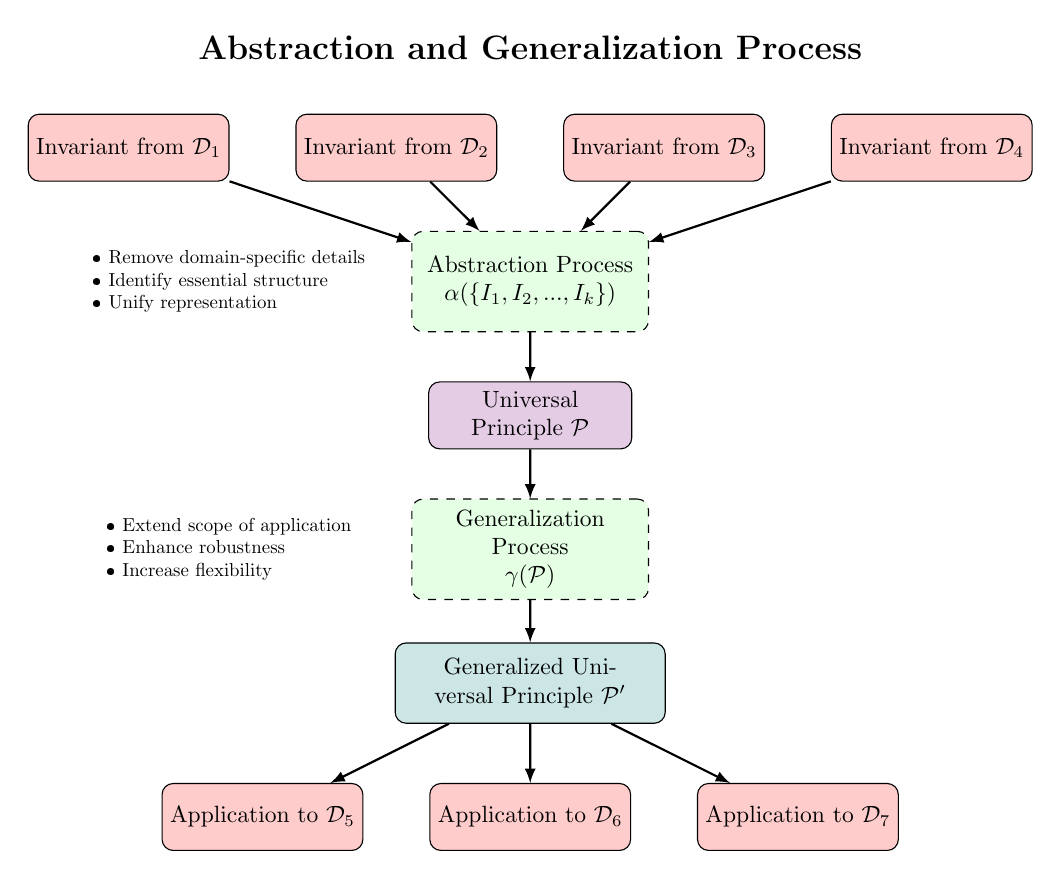
\begin{tikzpicture}[scale=0.85, transform shape]
    % Define styles
    \tikzset{
        invariantbox/.style={draw, fill=red!20, rounded corners, minimum width=3cm, minimum height=1cm, align=center},
        principlebox/.style={draw, fill=violet!20, rounded corners, minimum width=3cm, minimum height=1cm, text width=2.8cm, align=center},
        generalizedbox/.style={draw, fill=teal!20, rounded corners, minimum width=4cm, minimum height=1.2cm, text width=3.8cm, align=center},
        thickarrow/.style={->, >=latex, thick},
        processbox/.style={draw, dashed, fill=green!10, rounded corners, minimum width=3.5cm, minimum height=1.5cm, text width=3.3cm, align=center}
    }
    
    % Original invariants from domains
    \node[invariantbox] (i1) at (0,5) {Invariant from $\mathcal{D}_1$};
    \node[invariantbox] (i2) at (4,5) {Invariant from $\mathcal{D}_2$};
    \node[invariantbox] (i3) at (8,5) {Invariant from $\mathcal{D}_3$};
    \node[invariantbox] (i4) at (12,5) {Invariant from $\mathcal{D}_4$};
    
    % Abstraction process
    \node[processbox] (abstract) at (6,3) {Abstraction Process\\ $\alpha(\{I_1, I_2, ..., I_k\})$};
    
    % Arrows to abstraction
    \draw[thickarrow] (i1) -- (abstract);
    \draw[thickarrow] (i2) -- (abstract);
    \draw[thickarrow] (i3) -- (abstract);
    \draw[thickarrow] (i4) -- (abstract);
    
    % Universal principle
    \node[principlebox] (p) at (6,1) {Universal Principle $\mathcal{P}$};
    
    % Arrow from abstraction to principle
    \draw[thickarrow] (abstract) -- (p);
    
    % Generalization process
    \node[processbox] (generalize) at (6,-1) {Generalization Process\\ $\gamma(\mathcal{P})$};
    
    % Arrow from principle to generalization
    \draw[thickarrow] (p) -- (generalize);
    
    % Generalized principle
    \node[generalizedbox] (pg) at (6,-3) {Generalized Universal Principle $\mathcal{P}'$};
    
    % Arrow from generalization to generalized principle
    \draw[thickarrow] (generalize) -- (pg);
    
    % New domain applications
    \node[invariantbox] (d5) at (2,-5) {Application to $\mathcal{D}_5$};
    \node[invariantbox] (d6) at (6,-5) {Application to $\mathcal{D}_6$};
    \node[invariantbox] (d7) at (10,-5) {Application to $\mathcal{D}_7$};
    
    % Arrows to new applications
    \draw[thickarrow] (pg) -- (d5);
    \draw[thickarrow] (pg) -- (d6);
    \draw[thickarrow] (pg) -- (d7);
    
    % Abstraction details
    \node[align=left, scale=0.8] at (1.5,3) {
        \textbullet\ Remove domain-specific details\\
        \textbullet\ Identify essential structure\\
        \textbullet\ Unify representation
    };
    
    % Generalization details
    \node[align=left, scale=0.8] at (1.5,-1) {
        \textbullet\ Extend scope of application\\
        \textbullet\ Enhance robustness\\
        \textbullet\ Increase flexibility
    };
    
    % Title
    \node at (6,6.5) {\Large\textbf{Abstraction and Generalization Process}};
    
\end{tikzpicture}
\caption{The abstraction and generalization process for universal principles. Domain-specific invariants are first abstracted into a universal principle by eliminating domain-specific details while preserving essential structure. The principle is then generalized to expand its applicability beyond the original domains, enabling application to entirely new domains without prior exposure.}
\label{fig:abstraction_generalization}
\end{figure}